\section{Universal Verification Methodology}
\label{uvm}
The universal verification methodology (UVM) is an IEEE industry standard for the verification of design components \cite{uvmAccelleraScope}. It is developed by the Accellera group and its members. The goal is to create a modular, scalable and reusable generic verification environment. For these reasons, this methodology will be used for the verification of the SoC and its components. A short description of UVM will now be given.

UVM is based upon a hierarchy structure laid out by Accellera. This specifies guidelines for the creation of a verification environment and gives the support structure for this development. It does this by supplying a framework, for the designers to build on top of. This framework has the most general and essential features (Reporting, handshake mechanisms etc.), such that they do not need to be redeveloped for each project. This also ensures uniformity in testbench creation across many different work groups. The framework hierarchy is seen in figure \ref{fig:uvm_hierarchy} as it is laid out by Accellera \cite{uvmUserGuide}. Here the UVM agent can be expanded as it contains a sequencer, a driver, and a monitor. The expanded UVM agent can be seen in figure \ref{fig:uvm_agent}. Even though this is the recommended structure and should fit the most common use cases, the framework can be customized. 

\begin{figure}[H]
    \centering
    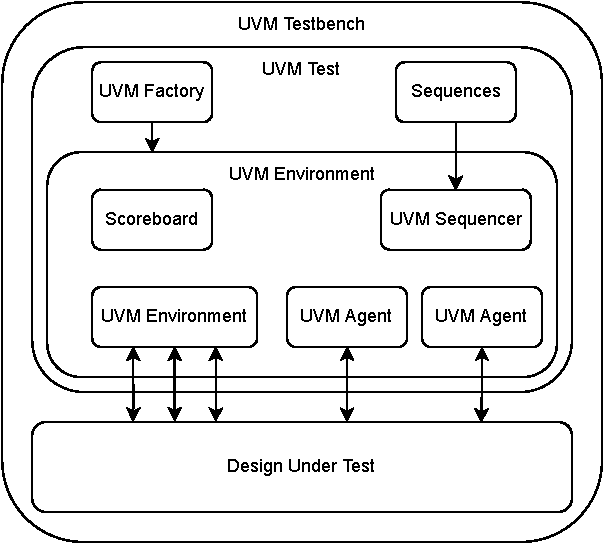
\includegraphics[width=0.6\linewidth]{subfiles/imgs/uvmHierarchy.drawio.pdf}
    \caption{Shows the complete hierarchy of the UVM structure laid out by Accellera.}
    \label{fig:uvm_hierarchy}
\end{figure}

\begin{figure}[H]
    \centering
    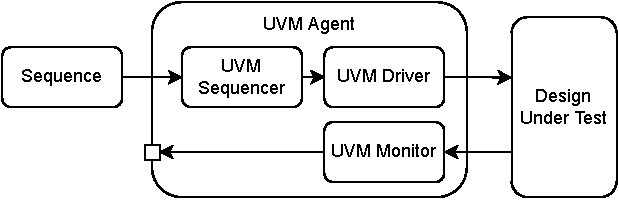
\includegraphics[width=0.6\linewidth]{subfiles/imgs/uvmAgentHierarchy.drawio.pdf}
    \caption{Shows the UVM components in a UVM agent and its connection to other components.}
    \label{fig:uvm_agent}
\end{figure}

The communication between components is based on transaction-level modeling (TLM) and UVM items. The items are designed to fit the specific device under test (DUT). It contains the information necessary to create stimuli to the DUT and updating scoreboard and reference module. The item is sent between components using TLM.

Each of the hierarchy levels has a base class associated with them. It is on top of these base classes that the project-relevant components will be built. Each of these classes and their functionality is described below \cite{uvmUserGuide}. 

\begin{itemize}
    \item \textbf{Testbench:} is the root class and container for all that needs to be simulated and tested. Typically this instantiates the DUT and the connections between the test and the DUT.
    \item \textbf{Test:} is the top-level UVM component. It has 3 main functions. To instantiate the test environment, configure the environment via a configuration database or factory overrides and apply stimulus to the DUT via the UVM sequences. This enables the designer to not have multiple instances of the same environment with different configurations for different test cases. Instead, the environment can be configured from this top-level UVM component to perform those test cases without repeating code.
    \item \textbf{Environment:} is a UVM component that instantiates and contains other reusable verification components such as agents, scoreboards, and other environments. It is also here the different components are connected and configured for default use. 
    \item \textbf{Scoreboard:} is the verification component that compares the DUT to an implemented reference module. The scoreboard does this by receiving UVM items from the DUT via the UVM agent using TLM ports. It can then use the reference module as a predictor and compare that to the DUT. 
    \item \textbf{Agent:} is a hierarchical component that contains other UVM components. These are typically a sequencer, a driver, and a monitor. The agent can either be active or inactive. An agent is active when it can drive stimuli to the DUT, which requires the use of a driver and sequencer. An inactive agent only contains a monitor.
    \begin{itemize}
        \item \textbf{Sequencer:} controls the flow of sequence items from the multiple sequences to the driver, i.e. queues different sequence items according to a set of given parameters.
        \item \textbf{Driver:} receives sequence items from the sequencer and converts them from transaction-level stimuli into pin-level stimuli for the DUT. For example, it can take a parallel data packet and transmit it via input pins to the DUT using a specified protocol. 
        \item \textbf{Monitor:} samples the DUT interface to convert data from pin-level stimuli into transaction-level stimuli. This data is then broadcast to the rest of the UVM testbench. The monitor can perform some levels of processing internally. For example, it can receive pin-level stimuli and decipher them according to a chosen protocol. So instead of broadcasting all pin-level activity, it first converts it into a specified UVM item and then broadcasts that using TLM.
    \end{itemize}
    \item \textbf{Sequence:} makes up the core stimuli of the verification plan. A sequence can be made of multiple data items which can be used to create the scenarios for testing the DUT extensively. The items are eventually sent to a sequencer which will then queue it and send it to the driver. Multiple sequences can be connected to the same sequencer. The randomization tools in UVM are commonly used in creating data items such that there is a higher chance of discovering bugs. A sequence is not part of the component hierarchy. A sequence can contain other sequences, called a parent or virtual sequence.  
\end{itemize}

A UVM environment can be developed either in SystemVerilog or SystemC, most commonly SystemVerilog. The SystemC variant is still under development but is in working condition. In this project, it has been chosen to use SystemC.
